%\documentclass[a4paper,11pt,twoside]{report}
%\usepackage[italian]{babel}
%\usepackage[utf8]{inputenc}
%\usepackage{microtype}
%\usepackage{hyperref}
%\usepackage{indentfirst}
%\usepackage[binding=5mm]{layaureo}
%\usepackage[T1]{fontenc}
%\usepackage{amssymb}
%\usepackage{amsmath}
%\usepackage{graphicx}
%\usepackage{booktabs}
%\usepackage{array}
%\usepackage{tabularx}
%\usepackage{caption}
%\usepackage{amsmath}
%\usepackage{amsfonts}
%\usepackage{eufrak}
%\usepackage{braket}
%\usepackage{amsthm}

%\renewcommand{\vec}{\bm}

%\author{Monica~Cavallari}
%\title{Appunti di \\Meccanica Quantistica}
%\date{}

%\begin{document}
\section[Meccanica statistica quantistica]{Meccanica statistica in ambito quantistico dei gas ideali (continuo)} %Meccanica statistica in ambito quantistico dei gas ideali (continuo)
Lo stato $\psi$ di molte particelle si può scrivere con l' insieme dei numeri di occupazione\\
\begin{equation}
\psi= \{n_{k}\}
\end{equation}
dove k sono i numeri quantici che labellano gli autostati di energia di particella singola; e $n_{k}$ sono il numero di particelle  aventi k come numero quantico.
$n_{k}=0,1$ Fermi\\
$n_{k}=0,1,2...$ Bose\\
Allora l' autovalore dell'energia è dato da
\begin{equation}
E_{\psi}= E(\{n_{k}\})= \sum_{k} n_{k}\epsilon_{k}
\end{equation}
$\epsilon_{k}$ rappresenta l' energia corrispondente al gruppo di numeri quantici.\\
Il numero totale di particelle risulta essere:
\begin{equation}
N=\sum_{k} n_{k}
\end{equation}
definisco fugacità:
\begin{equation}
\lambda=e^{\beta\mu}
\end{equation}
dove
\begin{equation}
\beta=\dfrac{1}{k_{B}T}
\end{equation}
Nell' insieme grancanonico il potenziale grancanonico è la trasformata di Legendre dell' energia rispetto alla temperatura e al potenziale chimico.

L'equazione del potenziale grancanonico risulta essere:
\begin{equation}
-PV(T,\mu,V)= U-TS-N\mu 
\end{equation}
Si può anche scrivere:
\begin{equation}
\dfrac{PV}{k_{B}T}=lnZ(T,\mu,V)
\end{equation}
dove Z è la funzione di granpartizione
\begin{equation}
Z(T,\mu,V)=\sum_{\psi} e^{-\beta(E_{\psi}-\mu N_{\psi})}
\end{equation}
avevamo anche visto che:
\begin{equation}
\dfrac{1}{\beta} \dfrac{\partial lnZ}{\partial \mu }= N =\dfrac{\partial PV}{\partial \mu }
\end{equation}

Proseguendo il calcolo della funzione di granpartizione si ha:
\begin{equation}\begin{split}
\mathcal{Z}=\\
=\sum_{N=0}^{\infty }\lambda^{N} Z(T,\mu,V)=\\
=\sum_{N=0}^{\infty } e^{ \beta\mu N} \sum_{\{n_{k}\}} {\delta\left(\sum_{k}{n_k-N}\right)} e^{-\beta \sum_{k} n_{k}\epsilon_{k} }  =\\
=\sum_{N=0}^{\infty }{\sum_{\left\{n_k\right\}}{\delta\left(\sum_{k}{n_k-N}\right)}\prod_{k}{e^{\beta\mu n_k}e^{-\beta\epsilon_k n_k}}}=\\
=\sum_{N=0}^{\infty }{\sum_{\left\{n_k\right\}}{\delta\left(\sum_k{n_k-N}\right)}\prod_k{\left(e^{\beta\mu}e^{-\beta\epsilon_k}\right)^{n_k}}}=\\
\textrm{ la doppia sommatoria } \sum_{N=0}^{\infty } \sum_{\{n_{k}\}}  
\textrm{ equivale alla} \sum_{\{n_{k}\}} \textrm{ senza fissare N  } \\ 
=\sum_{\left\{n_k\right\}}{\prod_{k}{e^{-\beta\left(\epsilon_k-\mu\right)n_k}}}=\\
\textrm{usando la proprietà distributiva della somma rispetto al prodotto} \\
=\prod_k{\sum_{n_k}{e^{-\beta\left(\epsilon_k-\mu\right)n_k}}}=\\
=\prod_k{\sum_n{e^{-\beta\left(\epsilon_k-\mu\right)n}}}=\\
\textrm{ ora n è fissato } \\
\end{split}\end{equation}
si hanno quindi due casi:
\begin{equation}\begin{split}
\prod_k
\begin{cases}
1+e^{-\beta\left(\epsilon_k-\mu\right)}, & \textrm{fermioni} \\
\frac{1}{1-e^{-\beta\left(\epsilon_k-\mu\right)}}, & \textrm{bosoni}
\end{cases}
\end{split}\end{equation}
Si ha:
\begin{equation}\begin{split}
N=\frac{1}{\beta}\frac{\partial \ln{\left(\mathcal{Z}\right)}}{\partial \mu}=\sum_k{\left\langle n_k \right\rangle}
\end{split}\end{equation}
(ho ottenuto una sommatoria perché ho svolto il logaritmo di una produttoria) (N è numero termodinamico) e quindi
\begin{equation}\begin{split}
\left\langle n_k \right\rangle=
\begin{cases}
\frac{1}{e^{\beta\left(\epsilon_k-\mu\right)}+1}, & \textrm{fermioni}\\
\frac{1}{e^{\beta\left(\epsilon_k-\mu\right)}-1}, & \textrm{bosoni}
\end{cases}
\end{split}\end{equation}
Posso trovare l' energia termodinamica $$U=\sum_k{\epsilon_k\left\langle n_k \right\rangle}$$
Ora ho il numero medio e l' energia, allora ho tutto quello che mi serve. Quando faccio la somma su tutti i livelli di energia in realtà mi conviene usare la densità di stati:
\begin{equation}\begin{split}
D\left(k\right)=Z\frac{V}{\left(2\pi\right)^3}
\end{split}\end{equation}
D(k) è la densità di stato nello spazio K nel caso di particella libera.

 I miei numeri quantici sono i k ( vettori d' onda) e lo spin; allora la sommatoria su k diventa un integrale:
\begin{equation}\begin{split} 
\sum_{k}\rightarrow \int D(k)\,dk
\end{split}\end{equation}
Integro su tutti i valori di k ( non sono infiniti perché ho le condizioni al contorno che mi danno la zona di Brin Luen(?), zona in cui non si ripetono valori che producono lo stesso risultato dell'integrale).

Faccio un ulteriore cambio di variabile usando lo jacobiano:
\begin{equation}\begin{split} 
\sum_{k}\rightarrow \int D(k)\,dk \\
\rightarrow \int D(E)\,dE 
\end{split}\end{equation}
dove E è:
\begin{equation}
E=\dfrac{\hbar^{2}k^2}{2m}
\end{equation}
Allora cambiando le variabili:
\begin{equation}\begin{split}
D\left(k\right)=Z\frac{V}{\left(2\pi\right)^3} \rightarrow D\left(E\right)=\frac{V}{2\pi^2}\left(\frac{2m}{\hbar ^2}\right)^{\frac{3}{2}}E^{\frac{1}{2}}
\end{split}\end{equation}
Ora calcolo N e U:
\begin{equation}\begin{split}
\sum_k\longrightarrow \int{D\left(\bar k\right)\textrm{d}\bar k}, \quad N\\
\int{D\left(E\right)\textrm{d}E}, \quad U
\end{split}\end{equation}
Si hanno quindi gli integrali fondamentali:
\begin{equation}\begin{split}
N=N_0+\int_{0}^{\infty }{D\left(E\right)\frac{1}{e^{\beta\left(E-\mu\right)}\pm 1} \textrm{d}E}
\end{split}\end{equation}
\begin{equation}\begin{split}
U=\int_{0}^{\infty }{D\left(E\right)E\frac{1}{e^{\beta\left(E-\mu\right)}\pm 1} \textrm{d}E}
\end{split}\end{equation}
$N_0$ è il numero di particelle sullo stato fondamentale.\\ Nel caso di Bose $N_0$ può essere infinito ( non deve valere il principio di Pauli quindi può anche essere un numero termodinamico).

Si possono verificare due situazioni:
\begin{itemize}
\item N fissato  (es. elettrone in un solido).
\item N non fissato  (es. fotone -> radiazione corpo nero, non so il numero di fotoni emessi).
\end{itemize}

\subsection{Piccola parentesi}
I fotoni sono Bosoni, soddisfano relazioni di commutazione. I Bosoni hanno polarizzazione (non spin 1) perpendicolare alla direzione di propagazione dovuta al gauge di Coulomb.

Evidenzio la differenza tra bosone e fermione nello scambio tra due particelle:\\
Fermioni: la funzione d' onda deve essere globalmente simmetrica.\\
Bosoni: la funzione d'onda deve essere antisimmetrica. In realtà si parla di campi (operatori). Se il campo commuta sono bosoni altrimenti fermioni. Dato che i fotoni mi danno un campo che commuta allora sono bosoni.

Se si fissa il numero $N$ si deve definire il potenziale chimico come $\mu=\mu\left(T,V,N\right)$.

Si verificano effetti differenti nel caso di Fermi e nel caso di Bose.
\subsection{Energia}
\begin{equation}
T_{F}k_{B}=E_{F}  \textrm{   fermi}  
\end{equation}
$T_{F}$ è la temperatura di fermi;\\
$E_{F}$ è l' energia di fermi:\\
I fermioni devono soddisfare il principio di esclusione di Pauli. Si inizia a riempire lo stato fondamentale. Una volta occupato questo avrà una degenerazione; per esempio se si trattasse di un atomo di idrogeno, gli elettroni potrebbero avere solo numero quantico principale e due valori dello spin, quindi sullo stato fondamentale ne posso mettere 2.
\begin{center}
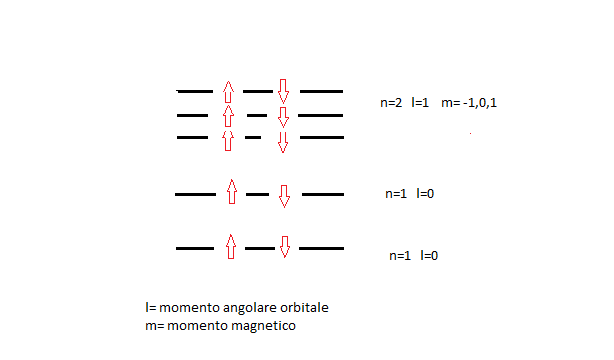
\includegraphics[scale=1]{immagini/occupazione-livelli.png}
\end{center}
Arriva un momento in cui tutti i livelli sono occupati:\\
\begin{equation}
\int_{0}^{E}D(E)E\,dE=N
\end{equation}
dove D(E) è la densità di energia.\\
Trovo:
\begin{equation}
E_{F}=\dfrac{\hbar^{2}}{2m}(\dfrac{3\pi^2N}{V})^{2/3}
\end{equation}
è un energia molto alta.
 \begin{equation}
T_{B}k_{B}=E_{B}  \textrm{  bose} 
\end{equation}

\subsection{Andamento Potenziale Chimico $\mu$}
Fermi:\\
All' inizio posso prendere $\mu=E_{F}$
\begin{center}
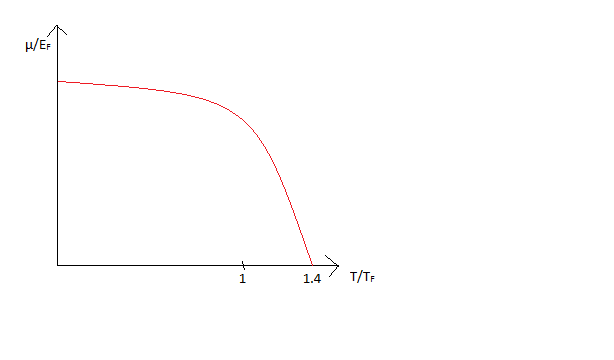
\includegraphics[scale=1]{immagini/pot-chimico-fermi.png} 
\end{center}
Bose:\\
All' inizio posso prendere $\mu=0$
\begin{center}
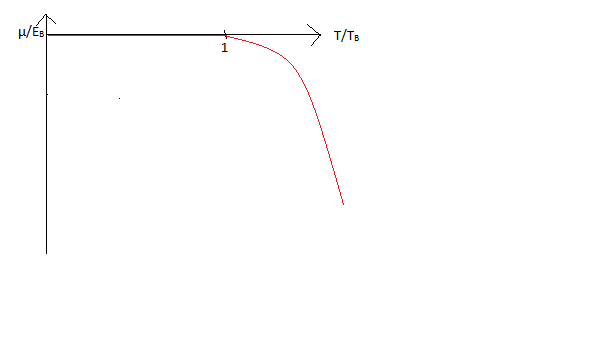
\includegraphics[scale=1]{immagini/pot-chimico-bose.png}
\end{center}

\subsection{Numero di occupazione medio ( in funzione dell'energia)}
Fermi: \\ Tutti gli elettroni cercano di occupare lo stato fondamentale.
Alzando la temperatura si svuotano i livelli sotto $E_{F}$ e si riempono quelli sopra.
\begin{center}
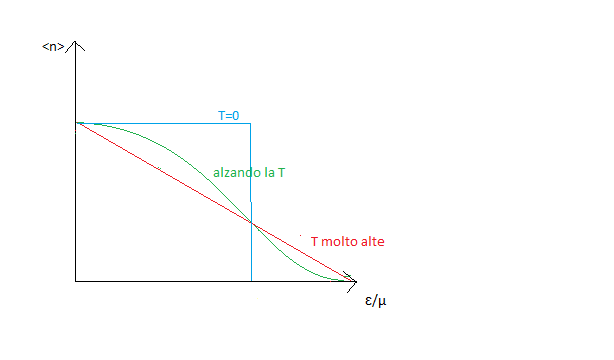
\includegraphics[scale=1]{immagini/n-occ-fermi.png}
\end{center}
Bose:\\ Aumentando T si svuota lo stato fondamentale e si riempono gli stati sopra.
Per T molto grande si ha uno svuotamento netto. Per T piccolo ho un addensamento a energia minima.
\begin{center}
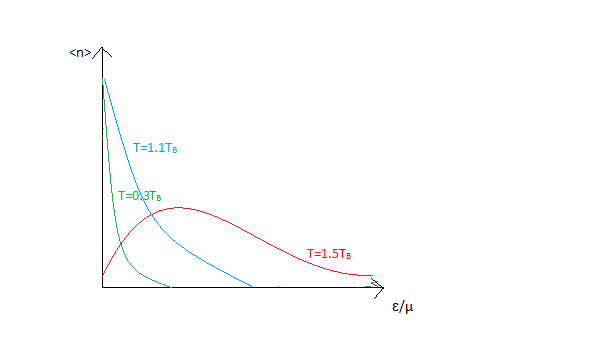
\includegraphics[scale=1]{immagini/n-occ-bose.png}
\end{center}
 
\subsection{Energia Bose}
La curva tende asintoticamente alla retta di Dulong-Petit.
\begin{center}
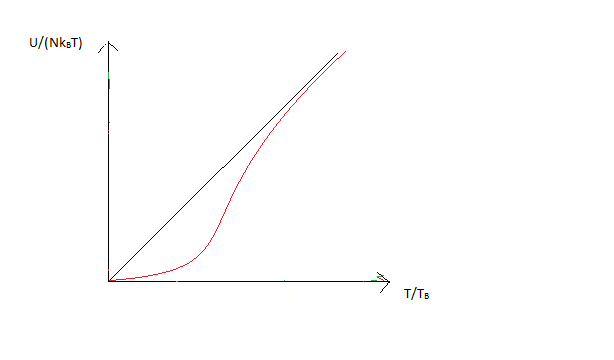
\includegraphics[scale=1]{immagini/energia-bose.png}
\end{center}

\subsection{Calore specifico Bose}
\begin{center}
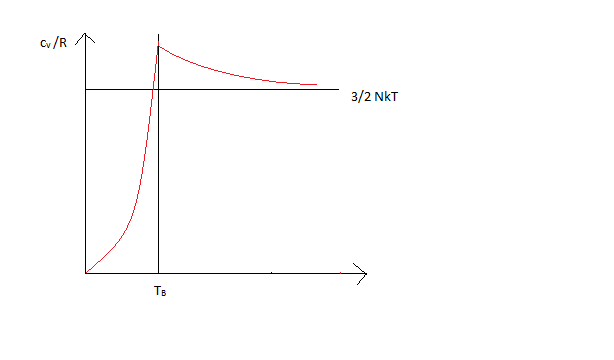
\includegraphics[scale=1]{immagini/calore-spec-bose.png}
\end{center}
Dove $c_{v}$ è il calore specifico e R è la costante dei gas. Da questo grafico si vede bene la transizione di fase. 
$N_{0}/N$ BOSE:
\begin{center}
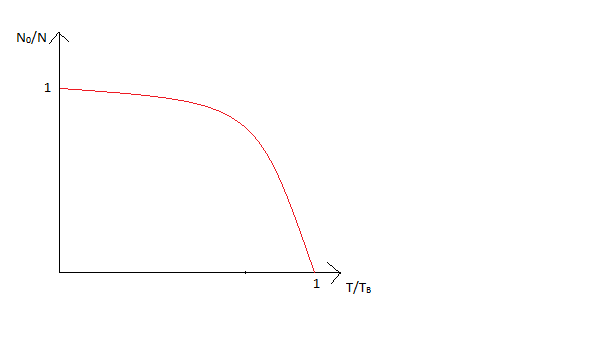
\includegraphics[scale=1]{immagini/ultimo-graf-bose.png}
\end{center}
Ho trovato che la termodinamica dei gas perfetti quantistici è determinato da 2 oggetti: il numero di occupazione medio del livello di energia e la densità di stati.
%\end{document}